\chapter{Chart types}
The chart library comes with the following chart plugins (types):
\begin{description}
\item[Bar] The bar chart plugin supports categories and subcategories, horizontal and vertical bar charts. It can also display stacked bar charts.
\item[Scatter] The scatter chart plugin supports single or multiple categories with two variables.
\item[Line] The line chart plugin supports categories and subcategories.
\item[Histogram] The histogram supports a multiple categories but no subcategories.
\item[Function] The function chart plugin supports plotting a single function with one or two variables.
\end{description}

Using these chart plugins it is possible to display all the relationships defined in Chapter 2.7. The following list describes how each relationship maps to a plugin appropriate for displaying the relationship.

\begin{description}
\item[Nominal comparison] Nominal comparisons should almost always be encoded as either bar or column charts.
\item[Time series] When there are few time time subdivisions and many categories, a line chart with a line for each category is a good solution. When there are few time subdivisions and few categories a column chart can be used. Finally, a time series with many time subdivisions should be encoded as a line chart.
\item[Ranking] A ranking relationship should be encoded as an ordered nominal comparison, and as such displayed in a bar or column chart.
\item[Part to whole] Part to whole relationships are best displayed as stacked bar or column charts.
\item[Deviation] When there are few categories a deviation relationship can be displayed as bars, and when there are many categories a line chart should be used.
\item[Distribution] When a distribution has a single variable and few values a histogram is recommended. When the distribution has a single variable and many values it should be displayed as a line chart. When the distribution has more than one variable, it is best to use a scatter chart.
\item[Correlation] Correlation relationships are best displayed as scatter charts.
\item[Function] Functions should be plotted using the plot chart, or if a function is very simple, a line chart.
\end{description}

Of course these solutions are only suggestions, as long as a chart plugin accepts the input it will try to draw the data. If that isn't sufficient it is always possible to extend either the available data relationships or add new chart plugins through an extension mechanism.

\section{Bar Chart}
\begin{figure}[H]
	\centering
	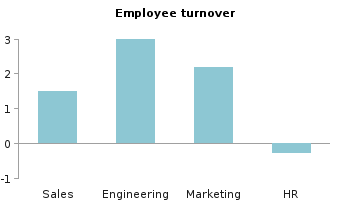
\includegraphics[width=.6\linewidth]{barsimple}
	\caption{Bar chart with single category}
\end{figure}

\begin{figure}[H]
	\centering
	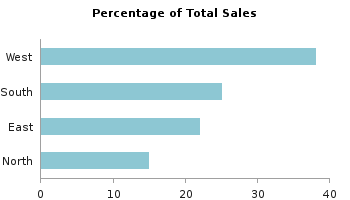
\includegraphics[width=.6\linewidth]{barrank}
	\caption{A ranking bar chart}
\end{figure}

\begin{figure}[H]
	\centering
	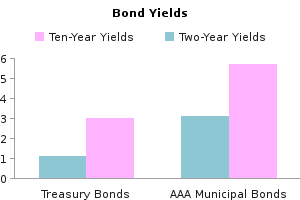
\includegraphics[width=.5\linewidth]{subcategory}
	\caption{A bar chart with subcategories and legend}
\end{figure}

\begin{figure}[H]
	\centering
	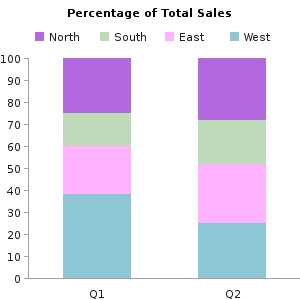
\includegraphics[width=.5\linewidth]{stacked}
	\caption{A bar stacked bar chart}
\end{figure}

\section{Scatter Chart}
\begin{figure}[H]
	\centering
	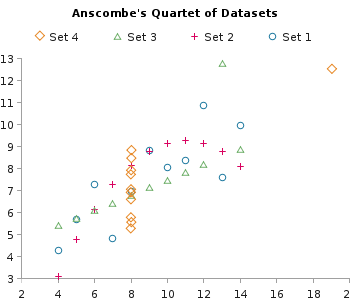
\includegraphics[width=.6\linewidth]{scatter}
	\caption{Scatter chart with multiple categories}
\end{figure}

\section{Line Chart}
\begin{figure}[H]
\centering
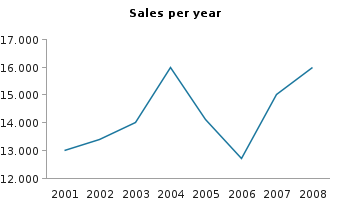
\includegraphics[width=.6\linewidth]{linesimple}
\caption{Line chart with single category}
\end{figure}

\begin{figure}[H]
\centering
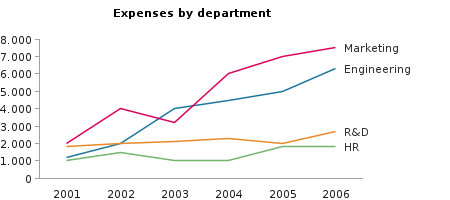
\includegraphics[width=.8\linewidth]{linemultiple}
\caption{Line chart with multiple categories}
\end{figure}

\section{Histogram}
\begin{figure}[H]
\centering
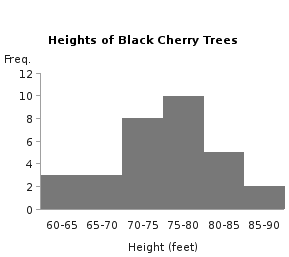
\includegraphics[width=.5\linewidth]{histogram}
\caption{Histogram with individual axis labels}
\end{figure}
\section{Function plotting}

Figure \ref{plots} shows: a) a simple plot of $y(t) = sin(t)$ and b) a plot of the "Rhodonea curve" defined by $r = cos(4\theta)$, plotted in polar coordinates. The sine plot also shows non-numeric and unicode support in labels.

\begin{figure}[H]
	\centering
	\subfloat[Sine wave]{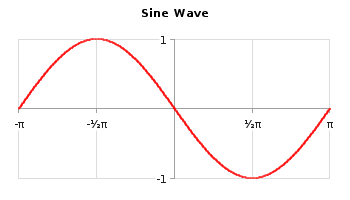
\includegraphics[width=0.5\textwidth]{sin}}
	\subfloat[Polar grid]{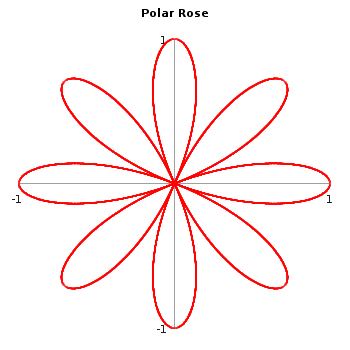
\includegraphics[width=0.5\textwidth]{rose}}
	\caption{Grid for cartesian and polar coordinate systems}
	\label{plots}
\end{figure}

\subsection{Plotting using interval arithmetic}
See \cite{shou05, fateman92, martin02}
